% ══════════════════════════════════════════════════════════════════════════════
% Lecture 12: Graphs – Representations, BFS, DFS
% ══════════════════════════════════════════════════════════════════════════════

% ══════════════════════════════════════════════════════════════════════════════
\section*{Graphs}
\addcontentsline{toc}{subsection}{Graphs – Representations, BFS and DFS}
% ══════════════════════════════════════════════════════════════════════════════

% ─────────────────────────────────────────────────────────────────────────────
\subsection{Definitions and Representations}

\begin{definition}{Graph}{graph}
A \textbf{graph} $G = (V, E)$ consists of a set of \textbf{vertices}
$V$ and a set of \textbf{edges} $E$ containing pairs (ordered or unordered)
of vertices. A graph can be \emph{undirected}, \emph{directed},
\emph{vertex-weighted}, \emph{edge-weighted}, etc.
\end{definition}

\begin{center}
\begin{tikzpicture}[font=\small, every node/.style={circle, draw, fill=blue!10,
                    inner sep=2pt, minimum size=0.6cm}]
  % Undirected graph
  \node (1u) at (0, 1.2) {1};
  \node (2u) at (1.4, 1.2) {2};
  \node (3u) at (2.8, 0.6) {3};
  \node (4u) at (1.4, 0) {4};
  \node (5u) at (0, 0) {5};
  \draw (1u)--(2u); \draw (1u)--(5u); \draw (2u)--(4u);
  \draw (3u)--(4u); \draw (4u)--(5u);
  \node[draw=none, fill=none] at (1.4, -0.7) {\textit{Undirected graph}};

  % Directed graph
  \begin{scope}[xshift=4.8cm, ->, >=Stealth]
  \node (1d) at (0, 1.4) {1};
  \node (2d) at (1.2, 1.4) {2};
  \node (3d) at (2.4, 1.4) {3};
  \node (4d) at (0, 0) {4};
  \node (5d) at (1.2, 0) {5};
  \node (6d) at (2.4, 0) {6};
  \draw (1d)--(2d); \draw (2d)--(3d);
  \draw (4d)--(5d); \draw (5d)--(6d);
  \draw (1d)--(4d); \draw (2d)--(5d); \draw (3d)--(6d);
  \node[draw=none, fill=none] at (1.2, -0.7) {\textit{Directed graph}};
  \end{scope}
\end{tikzpicture}
\end{center}

\subsubsection{Adjacency Lists}

We maintain an array $\mathit{Adj}$ of $|V|$ lists: the list for $u$ contains
all vertices $v$ such that $(u, v) \in E$. We denote this as $G.\mathit{Adj}[u]$ in
algorithms.

\begin{center}
\renewcommand{\arraystretch}{1.25}
\begin{tabular}{lll}
\toprule
\textbf{Operation} & \textbf{Cost} & \\
\midrule
Space & $\Theta(V + E)$ & compact for sparse graphs \\
List neighbors of $u$ & $\Theta(\deg(u))$ & \\
Test $(u,v) \in E$ & $O(\deg(u))$ & \\
\bottomrule
\end{tabular}
\end{center}

\subsubsection{Adjacency Matrix}

A $|V| \times |V|$ matrix where $a_{ij} = 1$ if $(i,j) \in E$, and 0 otherwise.

\begin{center}
\renewcommand{\arraystretch}{1.25}
\begin{tabular}{lll}
\toprule
\textbf{Operation} & \textbf{Cost} & \\
\midrule
Space & $\Theta(V^2)$ & dense, simple to implement \\
List neighbors of $u$ & $\Theta(V)$ & \\
Test $(u,v) \in E$ & $\Theta(1)$ & \\
\bottomrule
\end{tabular}
\end{center}

\begin{remark}{Choice of Representation}{graphrep}
Both representations can be extended to weighted graphs.
For \emph{sparse} graphs ($|E| \ll |V|^2$), adjacency lists are
preferable for space. The matrix is advantageous when edge membership
is tested frequently.
\end{remark}

% ─────────────────────────────────────────────────────────────────────────────
\subsection{Breadth-First Search (BFS)}

\begin{definition}{Breadth-First Search (BFS)}{bfs}
\textbf{Input:} graph $G = (V,E)$ (directed or undirected), source vertex $s \in V$.

\textbf{Output:} for every vertex $v$, $v.d$ = shortest distance (in number of
edges) from $s$ to $v$.
\end{definition}

\textbf{Idea:} send out a wave from $s$. It reaches all vertices at distance 1 first,
then at distance 2, etc. We use a \emph{queue} (FIFO).

\subsubsection{Pseudocode}

\begin{algorithm}[H]
\caption{BFS($G$, $s$)}
\begin{algorithmic}[1]
\For{each vertex $u \in G.V \setminus \{s\}$}
    \State $u.d \leftarrow \infty$
\EndFor
\State $s.d \leftarrow 0$
\State $Q \leftarrow \emptyset$;\; \textsc{Enqueue}$(Q, s)$
\While{$Q \ne \emptyset$}
    \State $u \leftarrow \textsc{Dequeue}(Q)$
    \For{each $v \in G.\mathit{Adj}[u]$}
        \If{$v.d = \infty$}           \AlgComment{$v$ not yet discovered}
            \State $v.d \leftarrow u.d + 1$
            \State \textsc{Enqueue}$(Q, v)$
        \EndIf
    \EndFor
\EndWhile
\end{algorithmic}
\end{algorithm}

\subsubsection{BFS Example}

Graph with 9 vertices $\{s, a, b, c, d, e, f, g, h\}$ from source $s$:

\begin{center}
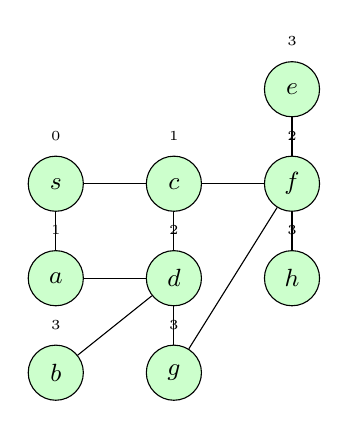
\begin{tikzpicture}[font=\small,
    node/.style={circle, draw, fill=blue!8, minimum size=0.7cm, inner sep=1pt},
    done/.style={circle, draw, fill=green!20, minimum size=0.7cm, inner sep=1pt}]
  % Layout matching the lecture slides
  \node[done] (s) at (0, 1.2) {$s$}; \node[above=2pt] at (s.north) {\tiny 0};
  \node[done] (a) at (0, 0)   {$a$}; \node[above=2pt] at (a.north) {\tiny 1};
  \node[done] (c) at (1.5,1.2){$c$}; \node[above=2pt] at (c.north) {\tiny 1};
  \node[done] (d) at (1.5,0)  {$d$}; \node[above=2pt] at (d.north) {\tiny 2};
  \node[done] (f) at (3.0,1.2){$f$}; \node[above=2pt] at (f.north) {\tiny 2};
  \node[done] (b) at (0,-1.2) {$b$}; \node[above=2pt] at (b.north) {\tiny 3};
  \node[done] (e) at (3.0,2.4){$e$}; \node[above=2pt] at (e.north) {\tiny 3};
  \node[done] (g) at (1.5,-1.2){$g$};\node[above=2pt] at (g.north) {\tiny 3};
  \node[done] (h) at (3.0,0)   {$h$}; \node[above=2pt] at (h.north) {\tiny 3};

  \draw (s)--(a); \draw (s)--(c);
  \draw (a)--(d); \draw (c)--(d); \draw (c)--(f);
  \draw (d)--(b); \draw (d)--(g);
  \draw (f)--(e); \draw (f)--(h); \draw (f)--(g);
\end{tikzpicture}
\end{center}

The discovery order is: $s \to a, c \to d \to f, b \to e, g, h$.
The final distances are indeed the distances in the graph.

\subsubsection{Analysis}

\begin{complexity}{BFS}{bfscplx}
\begin{itemize}[noitemsep]
  \item Each vertex is enqueued at most once: $O(V)$.
  \item Each edge is examined at most once (directed) or twice
        (undirected): $O(E)$.
  \item \textbf{Total complexity: $O(V + E)$.}
\end{itemize}
\end{complexity}

\textbf{Note:} BFS does not necessarily visit all vertices (only those
reachable from $s$). One can record the \emph{BFS tree} by storing
the edge that discovered each vertex ($v.\pi \leftarrow u$).

% ─────────────────────────────────────────────────────────────────────────────
\subsection{Depth-First Search (DFS)}

\begin{definition}{Depth-First Search (DFS)}{dfs}
\textbf{Input:} graph $G = (V,E)$, directed or undirected.

\textbf{Output:} for every vertex $v$, two timestamps:
$v.d$ (\emph{discovery} time) and $v.f$ (\emph{finishing} time).
\end{definition}

\textbf{Idea:} explore each edge as far as possible before backtracking.
As soon as a vertex is discovered, we explore from it (unlike BFS which
explores nearby vertices first). We restart from a new undiscovered
vertex if necessary.

\subsubsection{Vertex Colors}

During execution, each vertex has a color:
\begin{itemize}[noitemsep]
  \item \textbf{WHITE}: undiscovered.
  \item \textbf{GRAY}: discovered but not finished (exploration in progress from it).
  \item \textbf{BLACK}: finished (everything reachable from it has been explored).
\end{itemize}

\subsubsection{Pseudocode}

\begin{algorithm}[H]
\caption{DFS($G$)}
\begin{algorithmic}[1]
\For{each vertex $u \in G.V$}
    \State $u.\mathit{color} \leftarrow \text{WHITE}$
\EndFor
\State $\mathit{time} \leftarrow 0$
\For{each vertex $u \in G.V$}
    \If{$u.\mathit{color} = \text{WHITE}$}
        \State \Call{DFS-Visit}{$G$, $u$}
    \EndIf
\EndFor
\end{algorithmic}
\end{algorithm}

\begin{algorithm}[H]
\caption{DFS-Visit($G$, $u$)}
\begin{algorithmic}[1]
\State $\mathit{time} \leftarrow \mathit{time} + 1$
\State $u.d \leftarrow \mathit{time}$             \AlgComment{discovery timestamp}
\State $u.\mathit{color} \leftarrow \text{GRAY}$
\For{each $v \in G.\mathit{Adj}[u]$}
    \If{$v.\mathit{color} = \text{WHITE}$}
        \State \Call{DFS-Visit}{$G$, $v$}
    \EndIf
\EndFor
\State $u.\mathit{color} \leftarrow \text{BLACK}$
\State $\mathit{time} \leftarrow \mathit{time} + 1$
\State $u.f \leftarrow \mathit{time}$             \AlgComment{finishing timestamp}
\end{algorithmic}
\end{algorithm}

\subsubsection{DFS Example}

Graph with 8 vertices $\{a,b,c,d,e,f,g,h\}$, timestamps $d/f$:

\begin{center}
\begin{tikzpicture}[font=\small,
    node/.style={circle, draw, fill=blue!8, minimum size=0.75cm, inner sep=1pt}]
  \node[node] (b) at (1.5, 2.4) {$b$}; \node[above=0pt] at (b.north) {\tiny 1/12};
  \node[node] (c) at (3.0, 2.4) {$c$}; \node[above=0pt] at (c.north) {\tiny 8/11};
  \node[node] (e) at (4.5, 2.4) {$e$}; \node[above=0pt] at (e.north) {\tiny 13/16};
  \node[node] (a) at (0,   1.2) {$a$}; \node[above=0pt] at (a.north) {\tiny 2/7};
  \node[node] (d) at (3.0, 0.8) {$d$}; \node[above=0pt] at (d.north) {\tiny 9/10};
  \node[node] (f) at (4.5, 1.2) {$f$}; \node[above=0pt] at (f.north) {\tiny 14/15};
  \node[node] (h) at (1.5, 0)  {$h$};  \node[above=0pt] at (h.north) {\tiny 3/4};
  \node[node] (g) at (3.0, 0)  {$g$};  \node[above=0pt] at (g.north) {\tiny 5/6};

  % Tree edges
  \draw[->, >=Stealth, keygreen, thick] (b)--(a);
  \draw[->, >=Stealth, keygreen, thick] (a)--(h);
  \draw[->, >=Stealth, keygreen, thick] (a)--(g);
  \draw[->, >=Stealth, keygreen, thick] (b)--(c);
  \draw[->, >=Stealth, keygreen, thick] (c)--(d);
  \draw[->, >=Stealth, keygreen, thick] (e)--(f);
  % Cross/forward edges
  \draw[->, >=Stealth, keyred, dashed] (c)--(f) node[midway, right, font=\tiny]{};
\end{tikzpicture}
\end{center}

The DFS forest here contains two trees rooted at $b$ (time 1) and $e$ (time 13).

\subsubsection{Analysis}

\begin{complexity}{DFS}{dfscplx}
\begin{itemize}[noitemsep]
  \item Each vertex is discovered exactly once: $\Theta(V)$.
  \item Each edge is examined exactly once (directed) or twice
        (undirected): $\Theta(E)$.
  \item \textbf{Total complexity: $\Theta(V + E)$.}
\end{itemize}
\end{complexity}

DFS produces a \textbf{DFS forest}: one or more trees, each originating
from a \textsc{DFS-Visit} call in the main loop.

% ─────────────────────────────────────────────────────────────────────────────
\subsection{Edge Classification (DFS)}

In a DFS, each edge $(u,v)$ can be classified according to its timestamps:

\begin{center}
\renewcommand{\arraystretch}{1.35}
\begin{tabular}{lll}
\toprule
\textbf{Type} & \textbf{Definition} & \textbf{Condition} \\
\midrule
\textbf{Tree edge}    & in the DFS forest & $v$ was WHITE when $(u,v)$ explored \\
\textbf{Back edge}    & $(u,v)$: $u$ is descendant of $v$ & $v.d < u.d < u.f < v.f$ \\
\textbf{Forward edge} & $(u,v)$: $v$ is descendant of $u$, \newline but not via tree & $u.d < v.d < v.f < u.f$ \\
\textbf{Cross edge}   & any other edge & $v.f < u.d$ \\
\bottomrule
\end{tabular}
\end{center}

\begin{remark}{Undirected Graphs}{undirected}
In the DFS of an \emph{undirected} graph, we only obtain tree edges and
back edges — never forward edges or cross edges. Indeed, if $(u,v)$ is examined
from $u$ and $v$ is already GRAY or BLACK, then $v$ is necessarily an ancestor
of $u$ in the current tree, which results in a back edge.
\end{remark}

% ─────────────────────────────────────────────────────────────────────────────
\subsection{Summary: BFS and DFS}

\begin{center}
\renewcommand{\arraystretch}{1.45}
\begin{tabular}{lll}
\toprule
& \textbf{BFS} & \textbf{DFS} \\
\midrule
Structure used & Queue (FIFO) & Stack (recursion) \\
Exploration order & By increasing distance & Depth-first \\
Main output & Distances $v.d$ from $s$ & Timestamps $v.d$, $v.f$ \\
Complexity & $O(V+E)$ & $\Theta(V+E)$ \\
Reaches whole graph & No (from $s$ only) & Yes (if looping through all vertices) \\
Applications & Shortest path (unweighted) & Topological sort, connected components \\
\bottomrule
\end{tabular}
\end{center}